\documentclass[titlepage]{jsarticle}
\usepackage[dvipdfmx]{graphicx}
\usepackage{h31ec-exp}
\makeatletter
\newcommand{\figcaption}[1]{\def\@captype{figure}\caption{#1}}
\newcommand{\tblcaption}[1]{\def\@captype{table}\caption{#1}}
\makeatother
\title{オートマトンのプログラミング}
\grade{3年32番}
\author{平田 蓮}
\team{第C班}
\date{2019年10月29日}
\expdate{2019年10月7日, 10月21日, 10月28日}
\coauthor{}

\begin{document}
\maketitle
\section{目的}
    本実験では, 擬似自動販売機回路のプログラムを作成し, プログラミングを通してオートマトンの
    考え方を理解する.

\section{有限オートマトン(Finite Automaton: FA)}
    オートマトンとは自動機械という意味であるが、工学で用いられる場合は、離散的な入力及び出力
    を持つ機械のモデルのことであり, 状態とその遷移という考え方で捉える.
    ある装置の動作を実現することを考えた場合に, 入出力をまず考えるが, それだけでは動作を実現することは
    できない. 出力を決定する要素として内部状態という考えが必要である.

    装置の取り得る内部状態の数が有限個の場合, その装置を有限オートマトンといい, その動作は次の5個の
    集合と関数で記述できる.

    \paragraph{FAに必要な集合と関数}
        上で述べた集合と関数を示す.

        \begin{itemize}
            \item $X$: 入力集合
            \item $Q$: 状態集合
            \item $Z$: 出力集合
            \item $\sigma$: 状態遷移関数 $\sigma(X, Q) \rightarrow Q$
            \item $\omega$: 出力関数 $\omega(X, Q) \rightarrow Z または \ \omega(Q) \rightarrow Z$
        \end{itemize}

    \subsection{状態遷移図}
        FAの動作を図で表すには状態遷移図を用いると良い.

        例として10円硬貨だけが使える30円切手自動販売機を考える.
        Cancelボタンを押すと払い戻しとする.

        \begin{itemize}
            \item $X$: \{10[円], Cancel\}
            \item $Q$: \{0[円], 10[円], 20[円]\} (初期状態: 0[円])
            \item $Z$: \{1[枚], 10[円], 20[円]\}
        \end{itemize}

        このFAの状態遷移図を図\ref{fig:例状態遷移図}に示す。

        \begin{figure}[ht]
            \centering
            
            \caption{30円切手自動販売機}
            \label{fig:例状態遷移図}
        \end{figure}

\section{練習問題}
    実験テキストの練習問題の状態遷移図を示す.

    (1) 10円硬貨だけが使用できる40円切手自動販売機. Cancelを押すと払い戻し.

    \begin{figure}[ht]
        \centering
        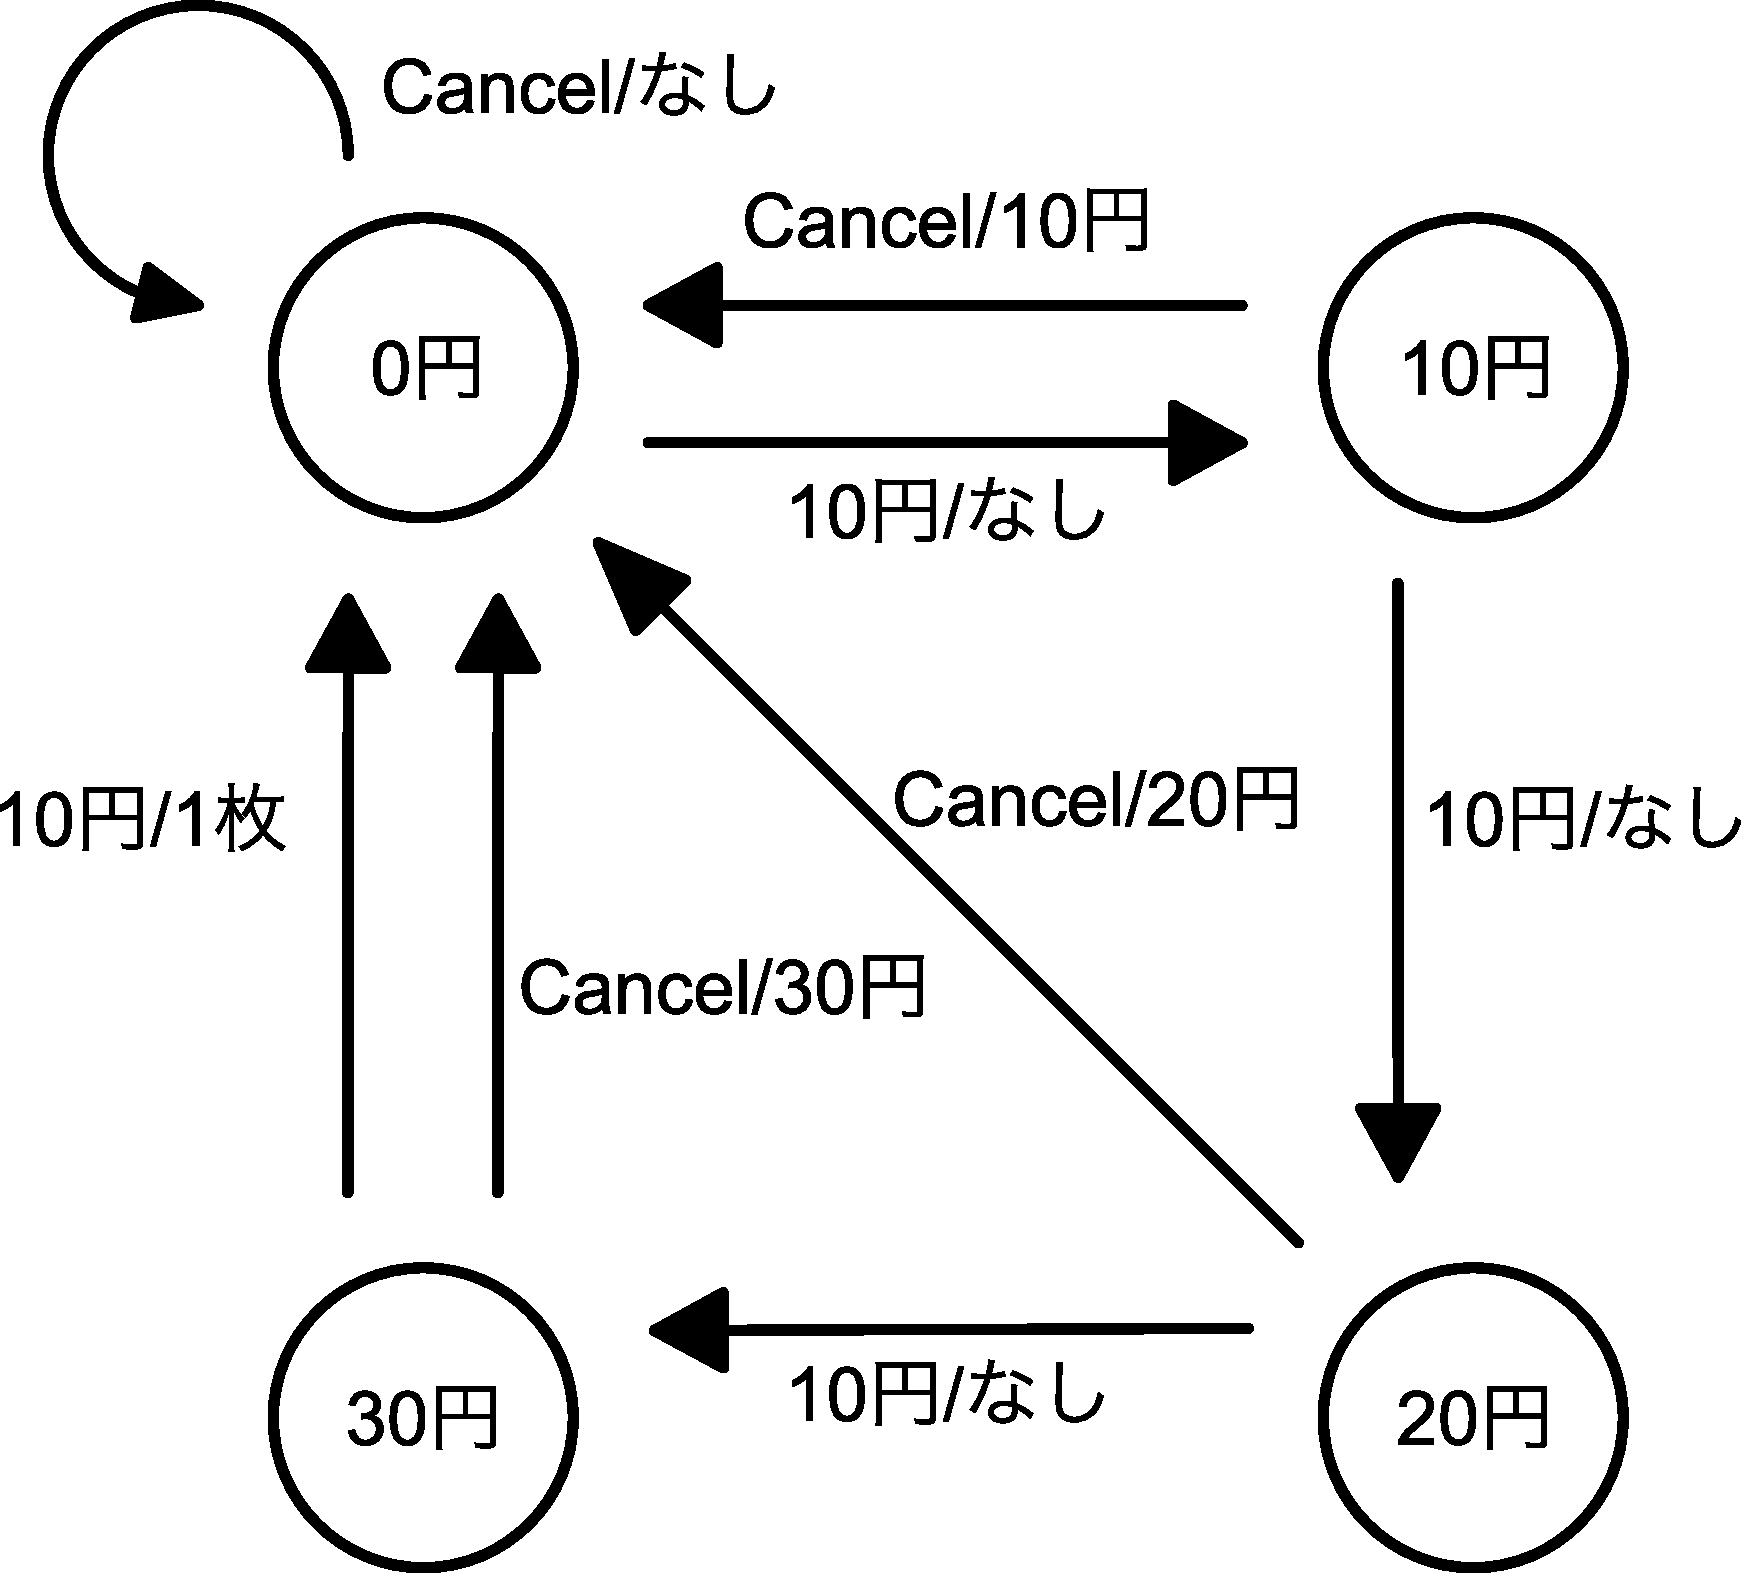
\includegraphics[width=8cm]{images/40.pdf}
        \caption{40円切手自動販売機}
        \label{fig:40状態遷移図}
    \end{figure}

    (2) 10円硬貨と50円硬貨だけ使える30円切手自動販売機. Cancelを押すと払い戻し.
    (お釣りはCancelを押さないと出てこない.)

    \begin{figure}[ht]
        \centering
        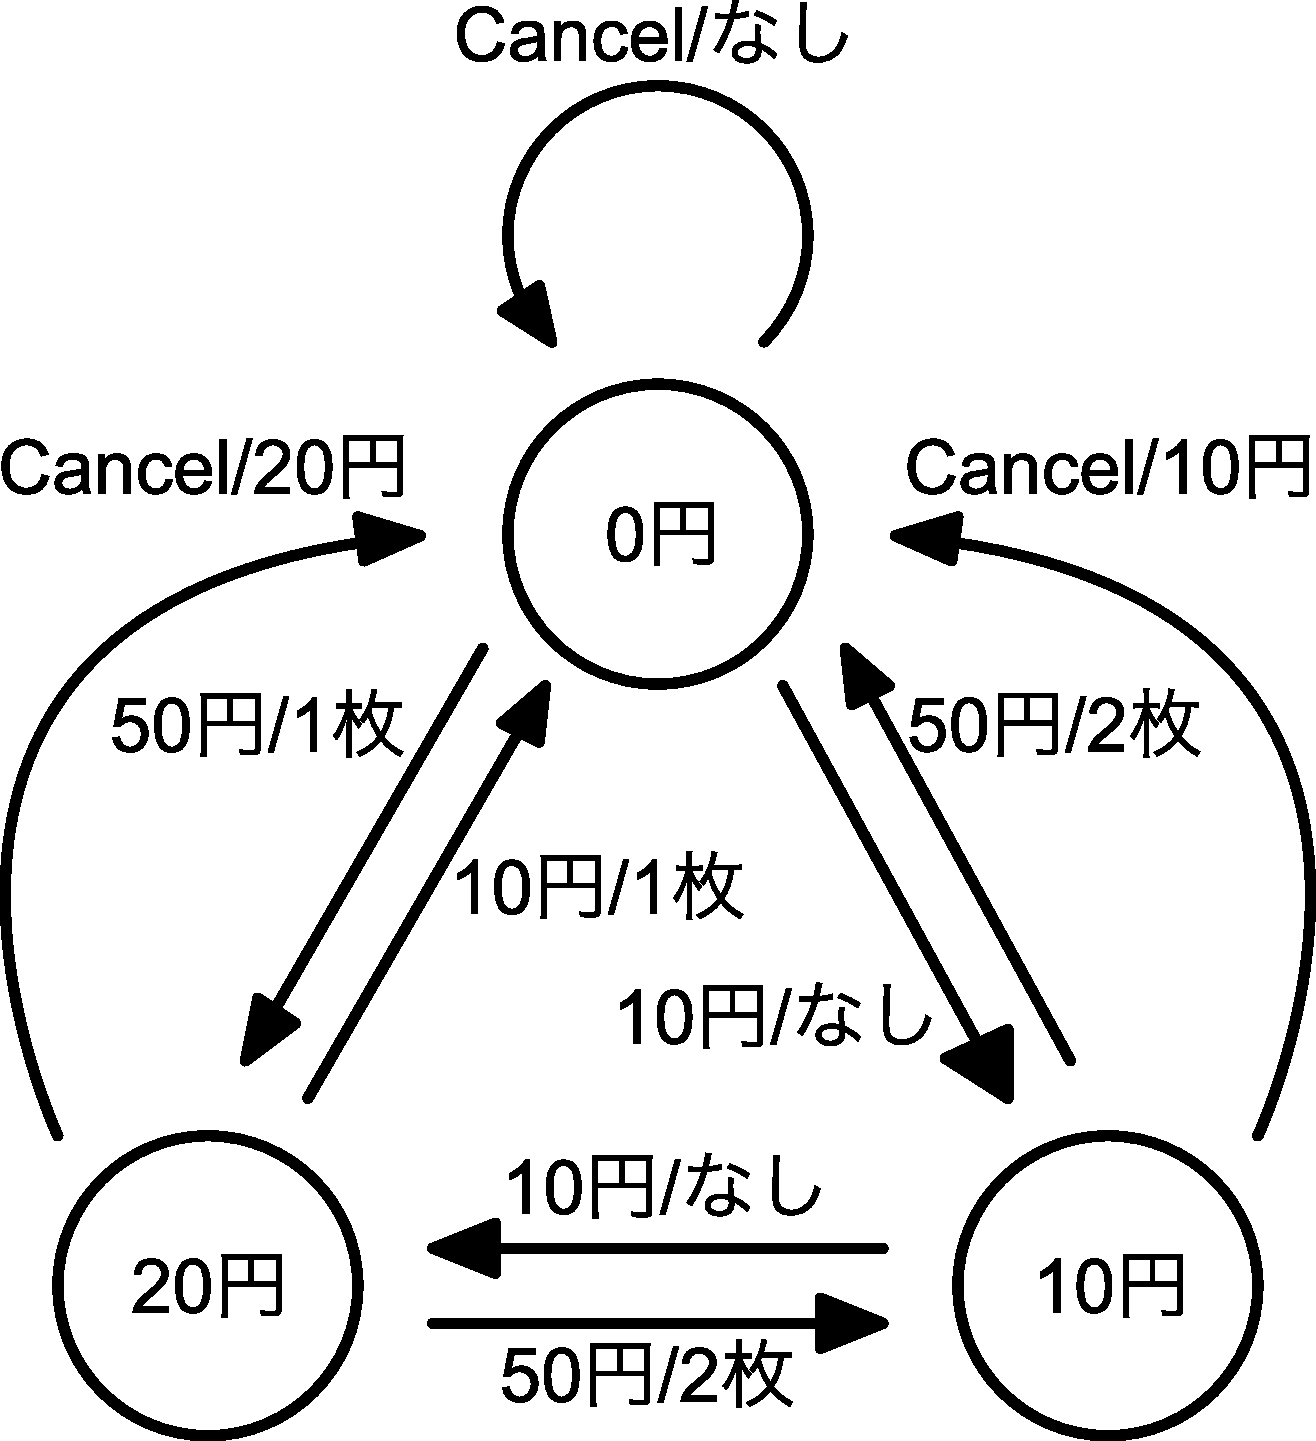
\includegraphics[width=8cm]{images/30.pdf}
        \caption{30円切手自動販売機}
        \label{fig:30状態遷移図}
    \end{figure}

    (3) 10円, 50円, 100円硬貨が使える20円切手自動販売機. Cancelを押すと払い戻し.
    (お釣りはCancelを押さないと出てこない.)

    \begin{figure}[ht]
        \centering
        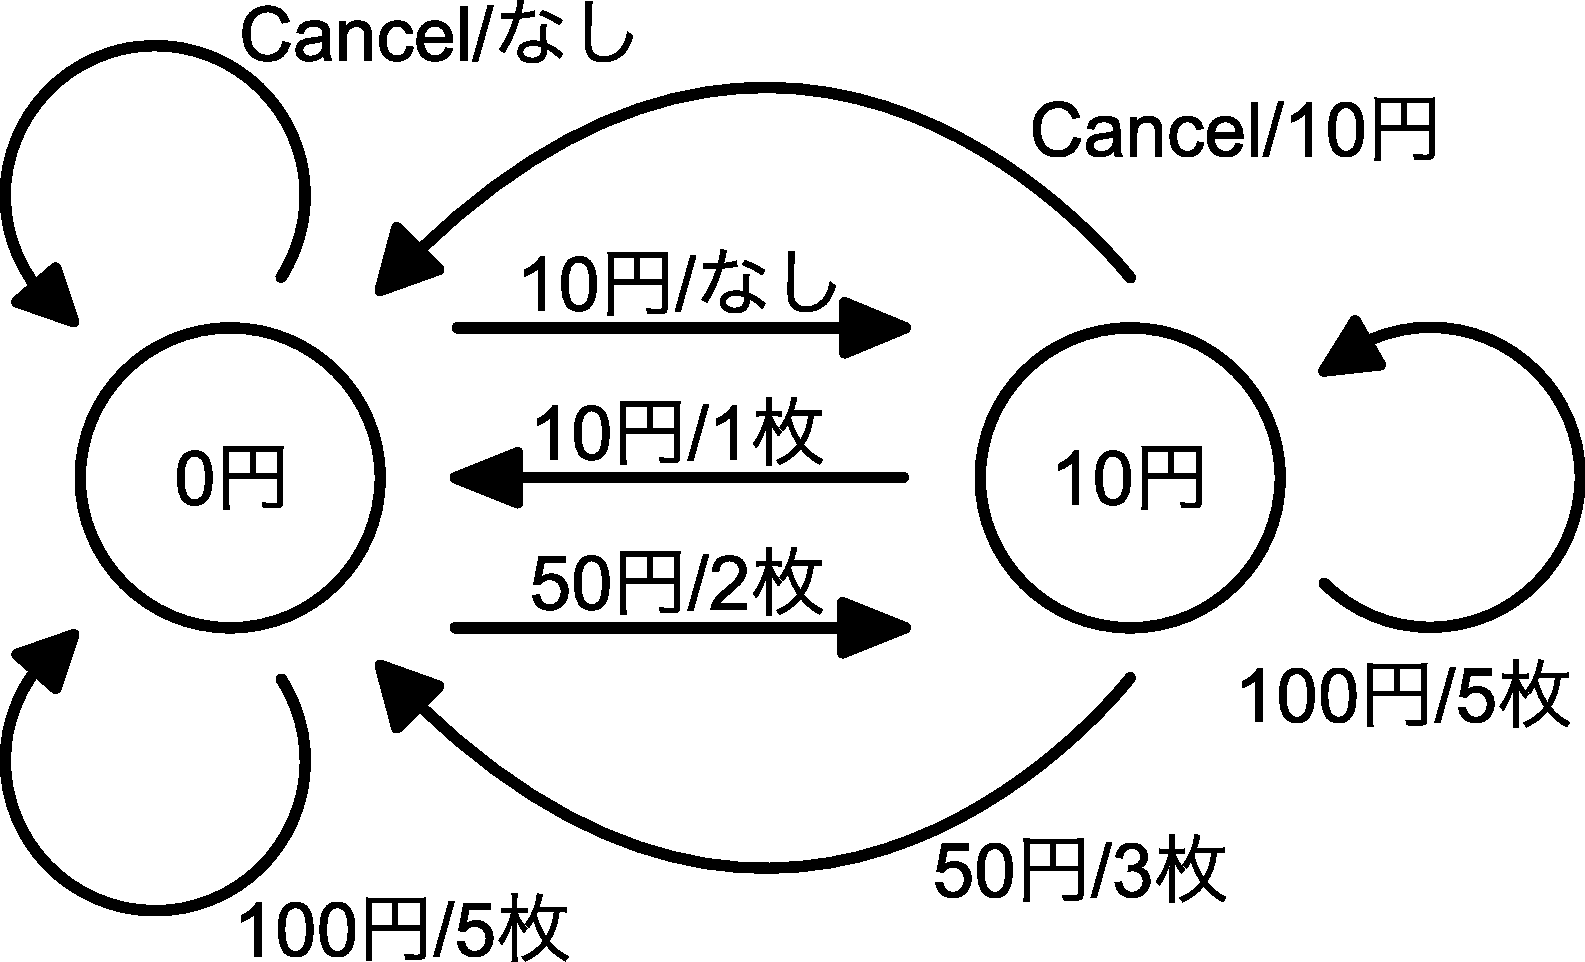
\includegraphics[width=8cm]{images/20.pdf}
        \caption{20円切手自動販売機}
        \label{fig:20状態遷移図}
    \end{figure}

\section{仮想自動販売機作成実習}
    今回は, 10円と50円が使える20円切手にした.
    10円入ってるときに50円を入れると60円になり切手が3枚出力されるので,
    3枚目は100円のランプを使うこととした.
    また, Cancelを押すと払い戻しをする.

    図\ref{fig:本番状態遷移図}に状態遷移図を示す.

    \begin{figure}[ht]
        \centering
        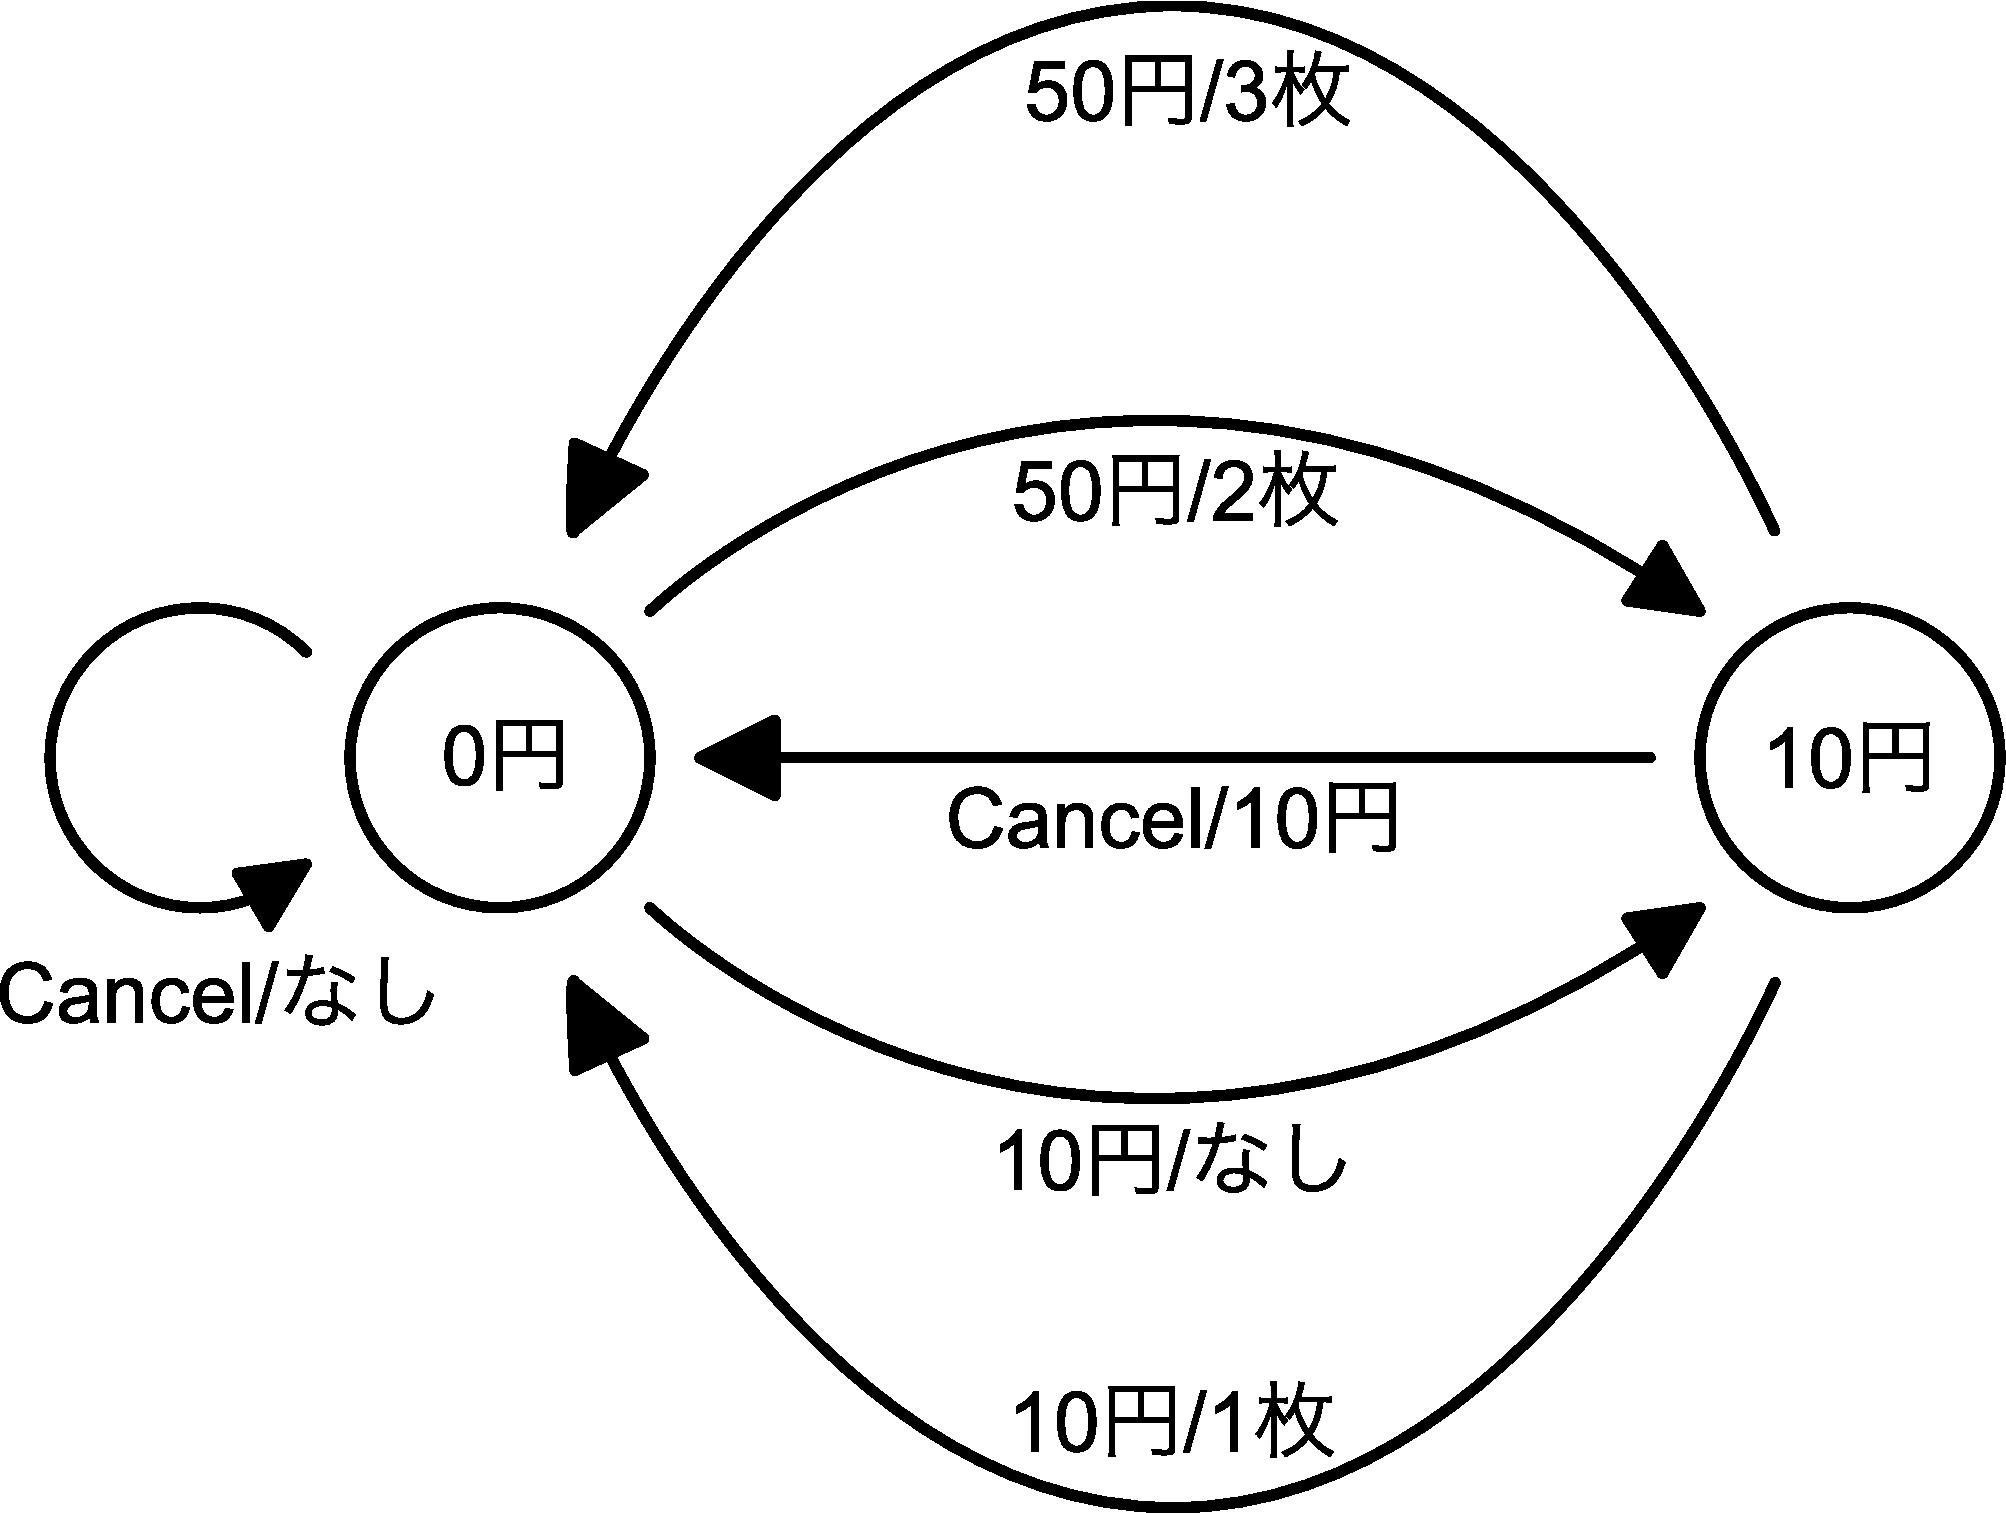
\includegraphics[width=8cm]{images/honban.pdf}
        \caption{20円切手自動販売機状態遷移図}
        \label{fig:本番状態遷移図}
    \end{figure}

    \subsection{ソースコード}
    
\section{調査課題「ワンチップマイコンについて調査せよ」}
    

\section{考察}
    

\section{感想}
    今回の実験では, 前期のディジタル論理回路の授業内容が活かせた.
    また, 今まで培ってきたプログラミング能力を駆使して比較的早く課題を終わらすことができた.
    発展課題には挑戦しなかったので, 今後機会があったら調べてみたい.

\begin{thebibliography}{99}
    \bibitem{フォトレジスタ} フォトレジスタ サヌキテックネット https://sanuki-tech.net/make-electronics/parts/cds-cell/
    \bibitem{フォトトランジスタ} フォトトランジスタの構造と特徴 光センサゼミナール http://www.kodenshi.co.jp/seminar/vol-02.html/
\end{thebibliography}

\end{document}
